\subsection{\label{sec:corrections}\desg{g12}-Specific Corrections}

\subsubsection{\label{sec:corrections.pcor}Final-State Particle Momentum Corrections}

The event reconstruction of a particle track in CLAS starts in region 1 of the DC after the track has gone through the target and start counter. To reconstruct the track back to the event vertex, additional energy loss from the target and start counter are included. The standard CLAS ELOSS package provides the required functionality as detailed in Ref. \cite{eloss}. ELOSS corrects for the energy lost as charged tracks go from the event vertex through the beam pipe, target, and start counter using the Bethe-Bloch equation \cite{pdg} to relate the material characteristics and path length to energy loss.

The momenta of the tracks as measured by the Drift-Chamber (\texttt{DC}) have a systematic shift within each sector as a function of azimuthal-angle $\phi$ of one of the tracks. This can be seen in the ``tranverse momentum balance'' plots shown in Fig.~\ref{fig:pbal.before}. The transverse momentum balance for a given particle is defined as the sum of the momentum of the other particles projected onto the line that is perpendicular to the beam having the same $\phi$ angle as the given particle minus its momentum transverse to the beam.

The procedure used is described in the \desg{CLAS} note for the momentum correction of the g9b dataset\cite{clas.note.g9bpcor}, though we choose to show the transverse (to the beam) momentum balance which is slightly more sensitive to this feature. The resulting transverse momentum and missing mass balance are shown in Figs.~\ref{fig.pbal} and \ref{fig:mmbal}. The latter plots can be compared directly to g9b's analysis.

The final \desg{g12} momentum corrections are in the clas6 trunk:
\begin{verbatim}
svn co https://jlabsvn.jlab.org/svnroot/clas/trunk/pcor/g12pcor
\end{verbatim}


The code to use the momentum corrections should look something like this:
\begin{verbatim}
#include "g12_pcor.hpp"

string parms_dir = "/group/clas/parms";

/// load up momentum correction parameters
clas6::g12::MomentumCorrection Pcor(parms_dir);

///begin loop over charged particles
{
    float newp = Pcor.pcor(oldp, phi, geant3_pid);
}
\end{verbatim}

Where geant3 pid is the particle ID (according to geant3) for \π[+], \π[-], p, \K[+] or \K[-].

\begin{figure}\begin{center}
\begin{subfigure}{0.4\columnwidth}
    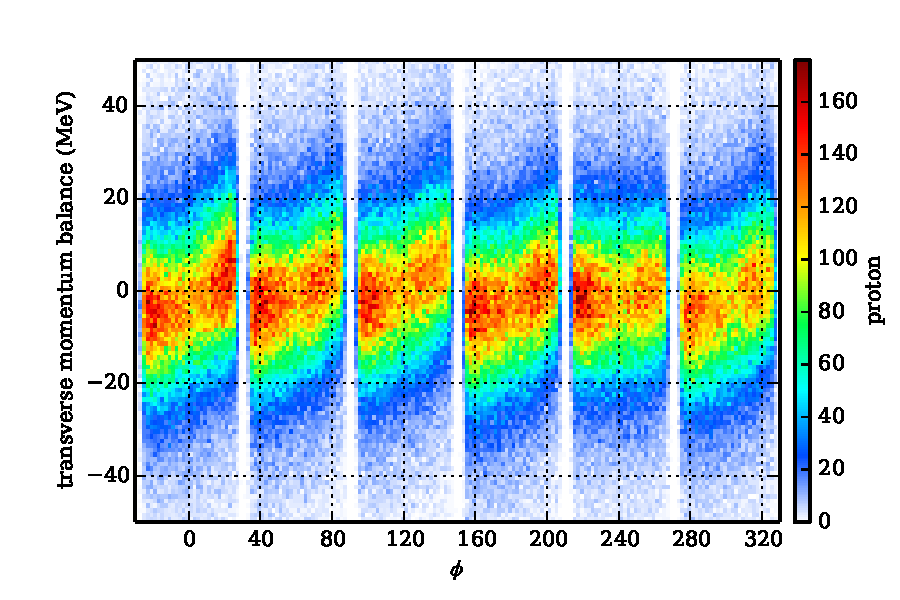
\includegraphics[width=\columnwidth]{figures/pcor/pcor_mptbal_p.pdf}
\end{subfigure}
\begin{subfigure}{0.4\columnwidth}
    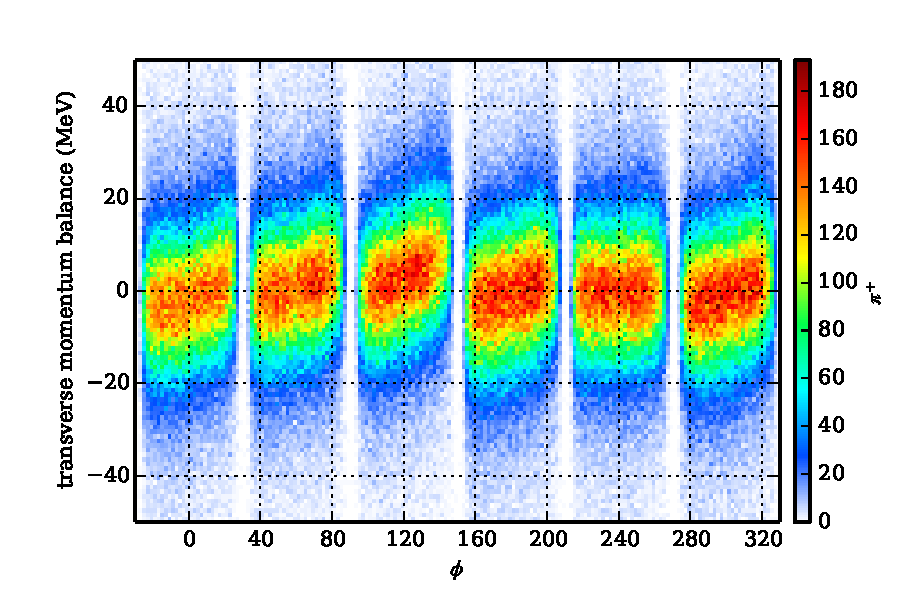
\includegraphics[width=\columnwidth]{figures/pcor/pcor_mptbal_pip.pdf}
\end{subfigure}
\begin{subfigure}{0.4\columnwidth}
    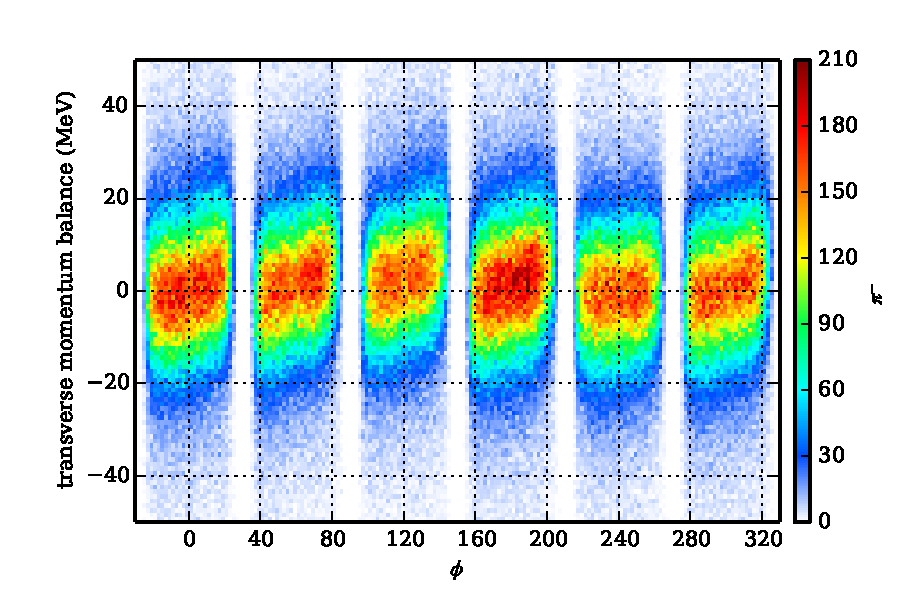
\includegraphics[width=\columnwidth]{figures/pcor/pcor_mptbal_pim.pdf}
\end{subfigure}
\caption[Momentum Balance Before Corrections]{\label{fig:pbal.before}Transverse momentum balance of exclusive p \π[+] \π[-] events as a function of azimuthal angle $\phi$ of each track before momentum corrections for the proton, π$^+$ and π$^-$.}
\end{center}\end{figure}

A simulataneous fit was done by adding a correction to the momenta of each particle for each sector which was linear in $\phi$. The result of the correction is shown in Fig.~\ref{fig:pbal_pcor}.

\begin{figure}\begin{center}
\begin{subfigure}{0.4\columnwidth}
    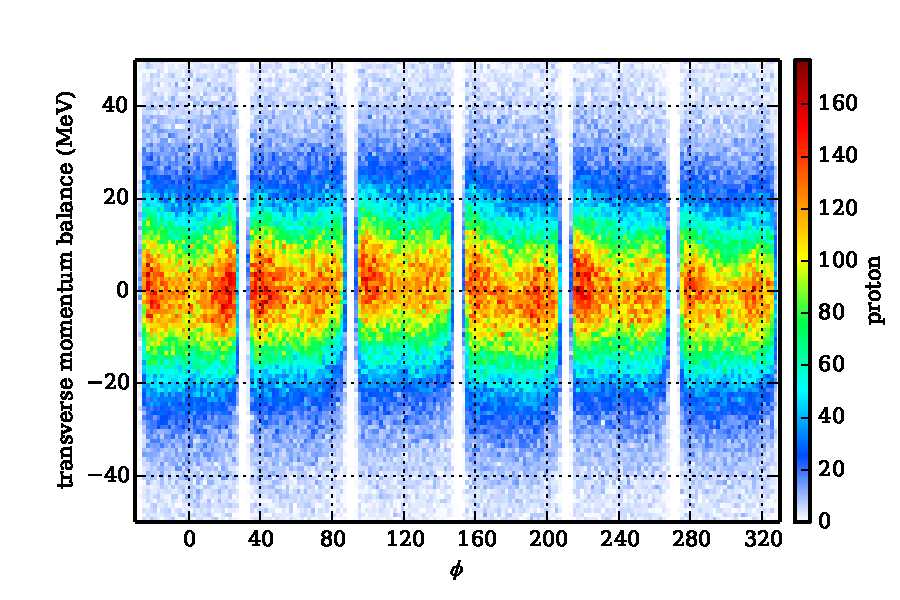
\includegraphics[width=\columnwidth]{figures/pcor/pcor_mptbal_fixed_p.pdf}
\end{subfigure}
\begin{subfigure}{0.4\columnwidth}
    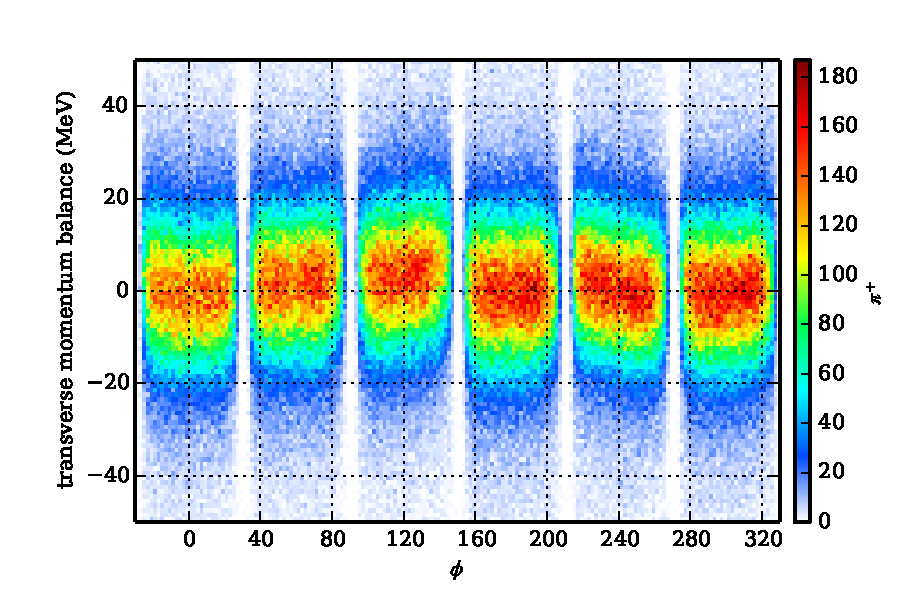
\includegraphics[width=\columnwidth]{figures/pcor/pcor_mptbal_fixed_pip.pdf}
\end{subfigure}
\begin{subfigure}{0.4\columnwidth}
    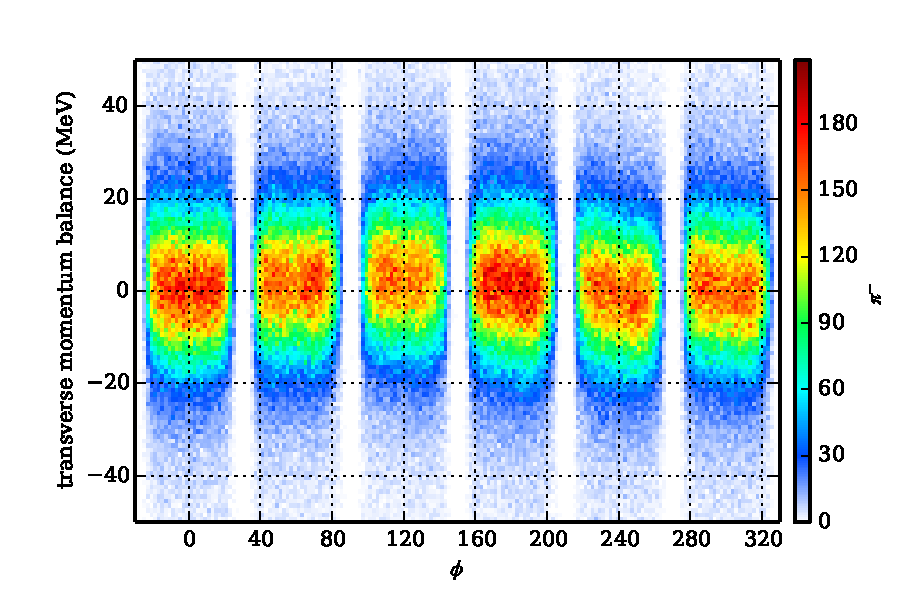
\includegraphics[width=\columnwidth]{figures/pcor/pcor_mptbal_fixed_pim.pdf}
\end{subfigure}
\caption[Momentum Balance Before Corrections]{\label{fig:pbal}Transverse momentum balance of exclusive p \π[+] \π[-] events as a function of azimuthal angle $\phi$ of each track after momentum corrections for the proton, π$^+$ and π$^-$.}
\end{center}\end{figure}

\begin{figure}\begin{center}
\begin{subfigure}{0.4\columnwidth}
    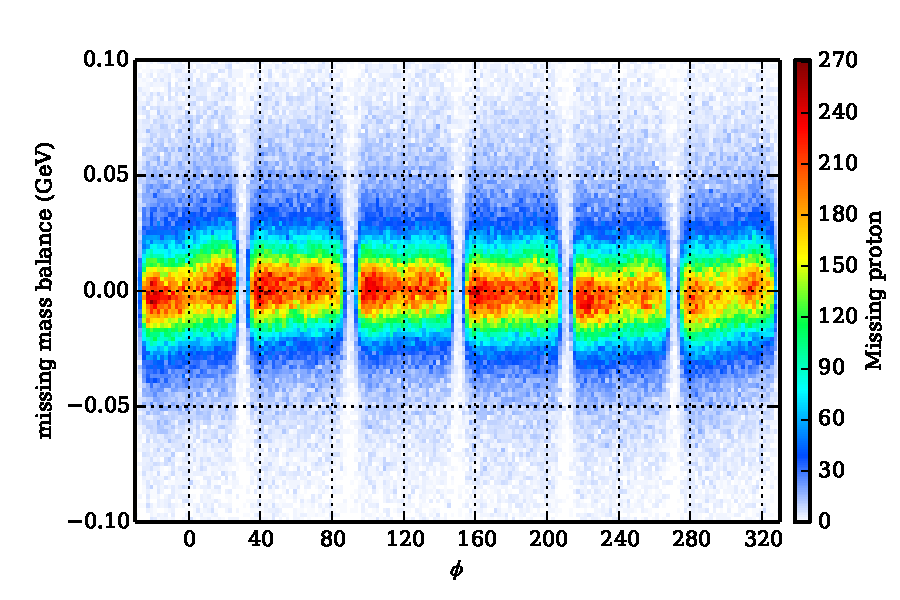
\includegraphics[width=\columnwidth]{figures/pcor/pcor_mpbal.pdf}
\end{subfigure}
\begin{subfigure}{0.4\columnwidth}
    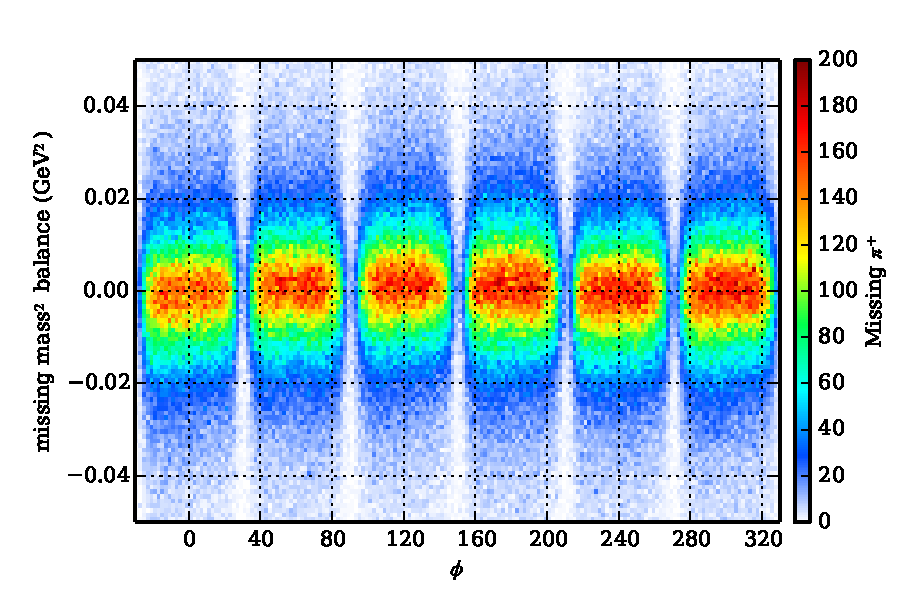
\includegraphics[width=\columnwidth]{figures/pcor/pcor_mpipbal.pdf}
\end{subfigure}
\begin{subfigure}{0.4\columnwidth}
    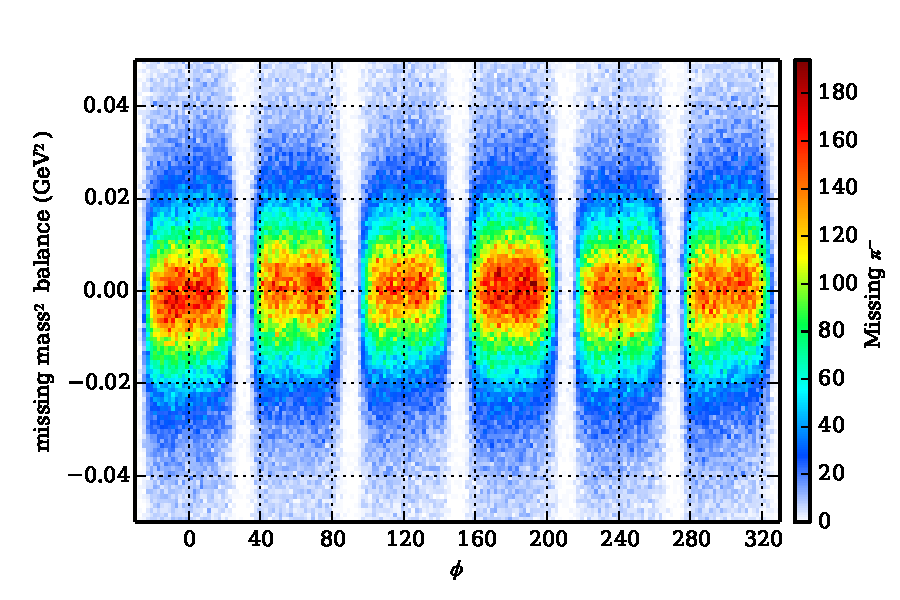
\includegraphics[width=\columnwidth]{figures/pcor/pcor_mpimbal.pdf}
\end{subfigure}
\caption[Momentum Balance Before Corrections]{\label{fig:mmbal}Missing mass (and mass-squared) balance of exclusive p \π[+] \π[-] events as a function of azimuthal angle $\phi$ of each track after momentum corrections for the proton, π$^+$ and π$^-$.}
\end{center}\end{figure}

\begin{figure}\begin{center}
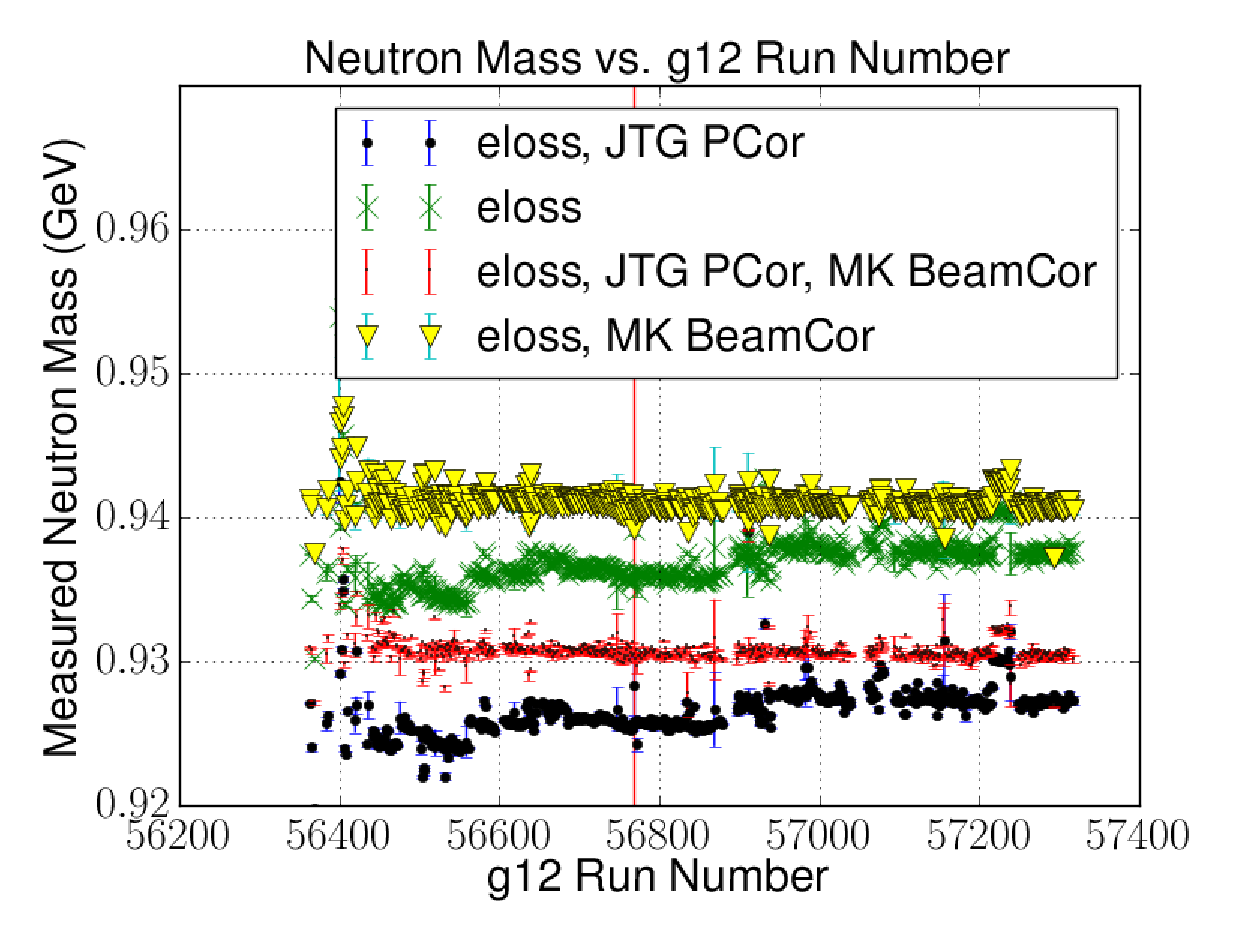
\includegraphics[width=0.6\columnwidth]{figures/corrections/C3pi_allcorr_neutron_rxr.eps}
\caption[Run by run Mass Balance Before and After Corrections]{\label{fig:mbal_pcor}Neutron mass balance of exclusive n \π[+] \π[+] \π[-] events as a function of run number for before corrections, momentum only, beam only, and after both beam and momentum corrections.}
\end{center}\end{figure}


\FloatBarrier
